\documentclass[aspectratio=169,t]{beamer}
\usepackage[utf8]{inputenc}
\usepackage[T1]{fontenc}
\usepackage[english]{babel}
\usepackage{hyperref}
\usepackage{tikz}

\usepackage{graphicx}
\usepackage{epstopdf}
\usepackage{multirow}

\usepackage{psfrag}
\usepackage{pgfplots}
\usepackage{framed}
\usepackage{xcolor}
\usepackage{booktabs}
\usepackage{caption}
\usepackage{epstopdf}
\usepackage{amsmath}
\usepackage{tabularx}
\usepackage[]{bookmark}
%\usepackage[3D]{movie15}
%\usepackage{media9}
\usepackage[binary-units,abbreviations]{siunitx}
\usepackage[textfont=normalsize, labelfont=normalsize, justification=centering]{subcaption}
\usepackage{marvosym}
\usepackage{calc}
\usepackage{color, colortbl}
\usepackage[]{svg} 
\usepackage[]{trfsigns} 
\usepackage[nomessages]{fp}
\usepackage[]{csquotes}\MakeOuterQuote{"}
\selectcolormodel{rgb}

\makeatletter
\def\beamer@calltheme#1#2#3{\def\beamer@themelist{#2}
	\@for\beamer@themename:=\beamer@themelist\do
	{\usepackage[{#1}]{\beamer@themelocation/#3\beamer@themename}}}
\def\usefolder#1{\def\beamer@themelocation{#1}}
\def\beamer@themelocation{}
\usefolder{theme}

\usetikzlibrary{matrix,
	decorations.pathreplacing,
	calc,
	positioning,
	external,
	3d,
	shapes,
	arrows,
	pgfplots.statistics}
\pgfplotsset{compat=1.16}
\tikzstyle{faunode}=[rounded corners, draw=faublue, fill=faublue!10,  align=center, inner sep=0.3cm, line width=0.4mm]
\tikzstyle{fauellipseFixedWidth}=[ellipse, draw=faublue, fill=faublue!10,  align=center, inner sep=0.3cm, line width=0.4mm, minimum width=3cm]
\tikzstyle{fauellipse}=[ellipse, draw=faublue, fill=faublue!10,  align=center, inner sep=0.3cm, line width=0.4mm]
\tikzstyle{fauarrow}=[draw=faublue,->, line width=0.4mm]
\tikzstyle{fauline}=[draw=faublue, line width=0.4mm]


\usepackage[backend=bibtex,sorting=none,doi=true,style=phys]{biblatex}
%\usepackage[]{biblatex}
\bibliography{./references}

% Themes:
%  - fau:          FAU theme
%  - fau-tf:       TechFak FAU theme
%  - fau-tf-lme:   TechFak LME FAU theme
%
% Options:
%  - image:        Cover image on title page
%  - plain:        Plain title page
%  - longtitle:    Title page layout for long title
\usetheme[longtitle]{fau-tf-lme}

% END of THEME SETTINGS
% --------------------------------------------------------------------------------------------------------------------------------------------------------------------------

\sisetup{
exponent-product =\ensuremath{{\,\cdot\,}}
}

% Enable semi-transparent animation preview
\setbeamercovered{transparent}
\setbeamertemplate{blocks}[rounded]
\captionsetup{labelformat=empty,labelsep=none, labelfont=normalsize, justification=centering}


\newcommand\Wider[2][1.0cm]{%
\makebox[\linewidth][c]{%
  \begin{minipage}{\dimexpr\textwidth+#1\relax}
  \raggedright#2
  \end{minipage}%
  }%
}


\let\origitem\item
\renewcommand{\item}{\normalfont\origitem}
\newcommand{\bluefat}[1]{\textcolor{faublue}{\textbf{#1}}}
\newcommand{\bolditem}{\normalfont\origitem\bfseries}
\newcommand{\question}{{\bf Question: }}
\newcommand{\answer}{{\bf Answer: }}
\newcommand{\myExample}{{\bf Example }}
\newcommand{\real}{\mbox{${\mathbb R}$}}
\definecolor{defColor}{rgb}{0.8,0.87,0.97}
\definecolor{defColorT}{rgb}{0,0,0}
\definecolor{defColorF}{rgb}{1,1,1}
\newenvironment{myDefinition}{%
	\def\FrameCommand{\fboxsep=\FrameSep{} \fcolorbox{defColorF}{defColor}}%
	\color{defColorT}\MakeFramed{\FrameRestore{}}}%
{\endMakeFramed}

% Title page
\title[Medical Engineering II]{Medical Engineering - Imaging Systems}
\author{Prof.\ Dr.-Ing.\ habil.\ Andreas Maier}
\date{SS 2021}
\institute{Pattern Recognition Lab (CS 5)}

\newcommand{\password}{\texttt{mt2\_ss21}}


\AtBeginSection[]{
	{
		\setbeamertemplate{footline}{}
		\begin{frame}[noframenumbering]{\insertsubtitle}
			 \tableofcontents[currentsection]
		\end{frame} 
	}
}
\AtBeginSubsection[]{
	{

		\setbeamertemplate{footline}{}
		\begin{frame}[noframenumbering]{\insertsubtitle}
			 \tableofcontents[currentsection, currentsubsection]
		\end{frame} 
	}
}


\usepackage{wrapfig}

%\newcommand{\bolditem}{\normalfont\origitem\bfseries}

\AtBeginSection[]{
    {
        \setbeamertemplate{footline}{}
        \begin{frame}[noframenumbering]{\insertsubtitle}
            \tableofcontents[currentsection]
        \end{frame} 
    }
}
\AtBeginSubsection[]{
    {

        \setbeamertemplate{footline}{}
        \begin{frame}[noframenumbering]{\insertsubtitle}
             \tableofcontents[currentsection, currentsubsection]
        \end{frame} 
    }
}

\subtitle{Phase Contrast X-ray}

\begin{document}

\frame[plain,c]{\titlepage} % plain-Option deaktiviert Kopf- und Fusszeile


%subtitle
%toc for this chapter


\section{Motivation}%
\label{sec:motivation}



\begin{frame}{Motivation: Frozen Mouse}
    \begin{center}\includegraphics[width=0.4\linewidth]{images/mouse-abs-updated.eps}\end{center}
    \begin{center}\includegraphics[width=0.4\linewidth]{images/mouse-dpc2-updated.eps}\end{center}
    \begin{center}\includegraphics[width=0.4\linewidth]{images/mouse-dark-field-updated.eps}\end{center}


    \begin{flushright}
        \tiny Sources: Erlangen Centre for Astroparticle Physics (ECAP), Erlangen, Germany
    \end{flushright}
\end{frame}

\begin{frame}{Motivation: A Cancerous  Mastectomy Sample}
    \begin{center}
        \begin{tabular}{lll}
            \includegraphics[width=0.3\linewidth]{images/MastectomyAbsorption.pdf} & \includegraphics[width=0.3\linewidth]{images/MastectomyPhaseContrast.pdf} &
            \includegraphics[width=0.3\linewidth]{images/MastectomyDarkfield.pdf}
        \end{tabular}
    \end{center}
    \vspace{-0.3cm}
    \begin{flushright}
        \tiny Sources: Erlangen Centre for Astroparticle Physics (ECAP), Erlangen, Germany
    \end{flushright}
\end{frame}

\begin{frame}{Contrast mechanisms in phase-contrast X-ray}
    \begin{itemize}
        \item \bluefat{Absorption}
              \begin{itemize}
                  \item based on differences in radiation absorption
                  \item excellent contrast where highly absorbing structures are embedded in relatively weakly absorbing material, i.e. bones and muscles\\[1cm]
              \end{itemize}
        \item \bluefat{Phase contrast}
              \begin{itemize}
                  \item of a light wave light based on differences in phase shifts
                  \item different weakly absorbing materials may exhibit a significant difference in the phase shifts\\[1cm]
              \end{itemize}
        \item \bluefat{Dark field}
              \begin{itemize}
                  \item based on ultra-small angle scattering
                  \item exhibits contrast for structural variations from structures with few micrometers diameters (fibers, grains)
              \end{itemize}
    \end{itemize}
\end{frame}

\section{Physics of Phase-contrast X-ray Imaging }%


%\begin{frame}{Refractive Index of X-rays}

%	\begin{itemize}
%		\item is a complex quantity
% 		\item is commonly written as: $n=1-\delta+i\beta$
% 		\item the real part $\delta$ causes the X-ray phase shift
% 		\item the imaginary part $\beta$ causes X-ray attenuation 
% 		\item $\beta$ is usually much smaller than $\delta$
% 	    \item close to one, thus
% 	    \begin{itemize}
% 	    \item X-ray lenses are not available
% 	    \item X-ray phase contrast imaging requires a different acquisition setup than phase contrast microscopy
% 	    \end{itemize} 
%\item can be calculated from atomic scattering factor. 
%\item The NIST database provides up-to-data information for  atomic scattering factor.

%	\end{itemize}


%\end{frame}

%\begin{frame}{Definition of a Wave}

%  \begin{align*}
%  \begin{split}
%  \psi(\mathbf{r}, t)  &= A(\mathbf{r}) e^{j\phi(\mathbf{r})} e^{j\omega t}\\
%  &=\psi_0 e^{jw(t-r/c)} e^{j(2\pi\delta/\lambda)r}e^{-(2\pi\beta/\lambda)r}
%  \end{split}  
%  \end{align*}

% \begin{itemize}
% \item $\lambda$: wavelength
% \item $\psi_0 e^{jw(t-r/c)}$: vacuum propagation
% \item $e^{j(2\pi\delta/\lambda)r}$: $\phi$-shift
% \item $e^{-(2\pi\beta/\lambda)r}$: decay
% \end{itemize}

% \end{frame}

\begin{frame}{Interferences}
    \begin{figure}
        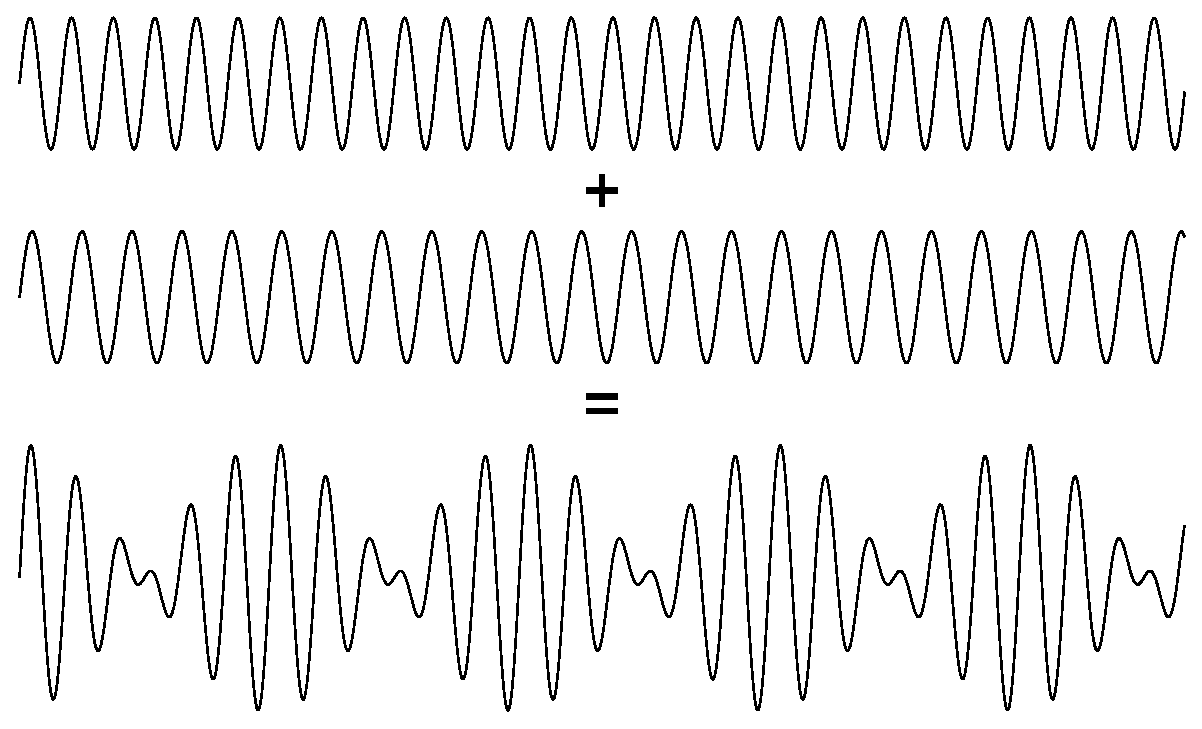
\includegraphics[height=0.8\textheight]{images/interferencesex.eps}
    \end{figure}

    \begin{flushright}
        \scriptsize Sources: Wilhelm Haas
    \end{flushright}
\end{frame}

\begin{frame}{Interferences}
    \begin{figure}
        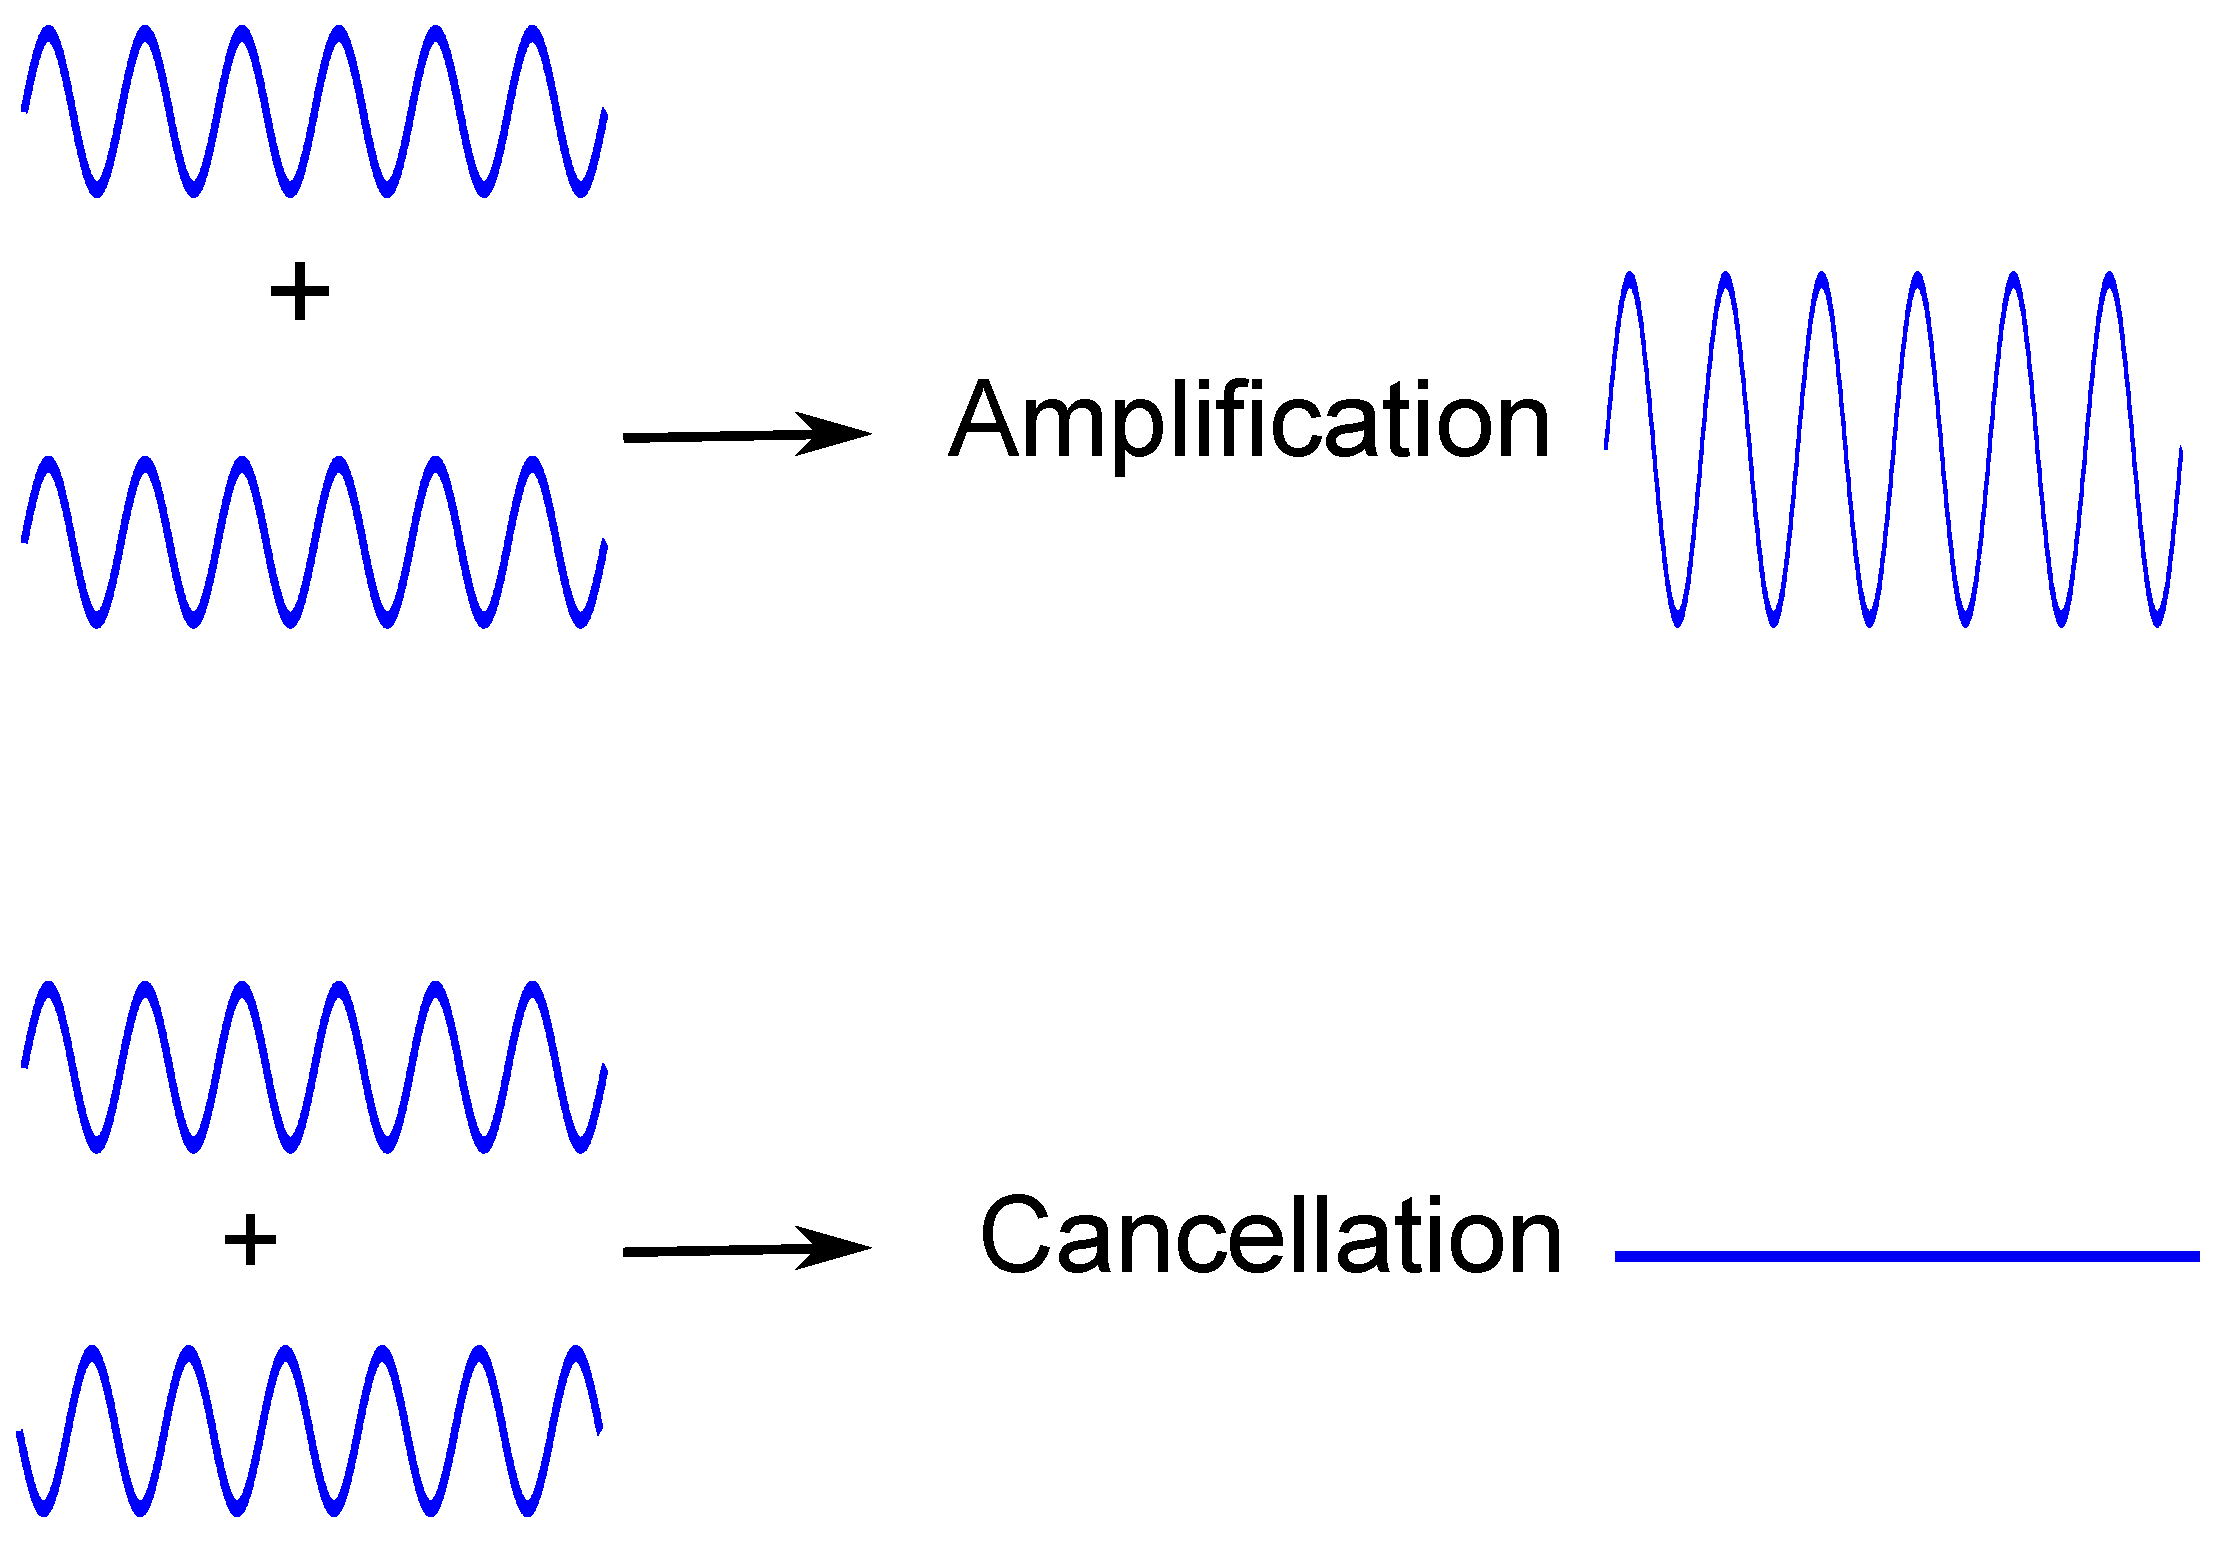
\includegraphics[height=0.8\textheight]{images/interferences3.eps}
    \end{figure}
\end{frame}

\begin{frame}[c]{Interference}
    Stationary interference requirements:
    \vspace{0.3cm}
    \begin{itemize}
        \setlength\itemsep{0.3cm}
        \item Need at least two waves
        \item Waves must have the \bluefat{same frequency}
        \item Waves must be in constant phase difference.
    \end{itemize}
\end{frame}


\begin{frame}[c]{Young's Double Slit Experiment}
    \begin{itemize}
        \setlength\itemsep{0.2cm}
        \item 1801: Thomas Young first demonstrated interference in light waves from two sources.
        \item Light is incident on a screen with a narrow slit
        \item The light waves emerging from this slit arrive at a second screen that contains two narrow, parallel slits.
    \end{itemize}

    \begin{figure}
        \centering{}
        \includegraphics[width=0.6\textwidth, trim={0  0 3.5cm 0},clip]{images/slit_book.pdf}
    \end{figure}
    \vspace{-0.4cm}
    \begin{flushright}
        \tiny Sources: Medical Imaging Systems: An Introductory Guide~\cite{bopp18}
    \end{flushright}
\end{frame}

\begin{frame}[c]{Young's Double Slit Experiment}
    \begin{figure}
        \centering{}
        \includegraphics[width=\textwidth]{images/slit_book.pdf}
    \end{figure}
    \begin{flushright}
        \tiny Sources: Medical Imaging Systems: An Introductory Guide~\cite{bopp18}
    \end{flushright}
\end{frame}

\begin{frame}[c]{Young's Double Slit Experiment}
    \begin{itemize}
        \setlength\itemsep{0.3cm}
        \item The light from the two slits form a visible pattern on a screen
        \item The pattern consists of a series of bright and dark parallel bands called \textit{fringes}
        \item Constructive interference occurs where a bright fringe occurs
        \item Destructive interference results in a dark fringe
    \end{itemize}
\end{frame}

\begin{frame}{Interference Patterns}
    \vspace{-1cm}
    \begin{columns}[c, onlytextwidth]
        \begin{column}{0.5\textwidth}
            \begin{itemize}
                \item Constructive interference occurs at the center point
                \item The two waves travel the same distance and arrive in phase, i.e. arrive at the same time.
            \end{itemize}
        \end{column}\begin{column}{0.5\textwidth}
            \begin{figure}
                \centering{}
                \includegraphics[height=1\textheight, trim={5cm  0 2cm 0},clip]{images/bright.pdf}
            \end{figure}
        \end{column}
    \end{columns}
\end{frame}

\begin{frame}{Interference Patterns}
    \vspace{-1cm}
    \begin{columns}[c, onlytextwidth]
        \begin{column}{0.5\textwidth}
            \begin{itemize}
                \item The upper wave has to travel farther than the lower wave
                \item The upper wave travels one wavelength farther
            \end{itemize}
        \end{column}\begin{column}{0.5\textwidth}
            \begin{figure}
                \centering{}
                \includegraphics[height=1\textheight, trim={2cm  0 2cm 0},clip]{images/bright2.pdf}
            \end{figure}
        \end{column}
    \end{columns}
\end{frame}

\begin{frame}{Interference Patterns}
    \vspace{-1cm}
    \begin{columns}[c, onlytextwidth]
        \begin{column}{0.5\textwidth}
            \begin{itemize}
                \item The upper wave travels one-half of a wavelength farther than the lower wave
                \item The trough of the bottom wave overlaps the crest of the upper wave ($180^\circ$ phase shift)
            \end{itemize}
        \end{column}\begin{column}{0.5\textwidth}
            \begin{figure}
                \centering{}
                \includegraphics[height=1\textheight, trim={2cm  0 2cm 0},clip]{images/bright3.pdf}
            \end{figure}
        \end{column}
    \end{columns}
\end{frame}

\begin{frame}{Interference Patterns}
    \vspace{-1cm}
    \begin{columns}[c, onlytextwidth]
        \begin{column}{0.5\textwidth}
            \begin{itemize}
                \item[$d$] Distance between slits S1 and S2
                \item[$\Delta d$] Path difference
            \end{itemize}
        \end{column}\begin{column}{0.5\textwidth}
            \begin{figure}
                \centering{}
                \includegraphics[height=1\textheight, , trim={2cm  0 2cm 0},clip]{images/bright4.pdf}
            \end{figure}
        \end{column}
    \end{columns}

\end{frame}

\begin{frame}[c]{Interference Patterns}
    \begin{itemize}
        \item \bluefat{Bright fringe:} path difference must be either zero or some integral multiple of of the wavelength
              \begin{eqnarray*}
                  \Delta d &=& d\sin\theta_{\text{bright}}= m\lambda
              \end{eqnarray*}
              where the order number is
              \begin{eqnarray*}
                  m &=& 0,\pm 1, \pm 2, \pm 3,\ldots
              \end{eqnarray*}
    \end{itemize}
\end{frame}

\begin{frame}[c]{Interference Patterns}
    \begin{itemize}
        \item \bluefat{Dark fringe:} path difference must be of an odd half wavelength
              \begin{eqnarray*}
                  \Delta d &=& d\sin\theta_{\text{dark}}= \left(m + \dfrac{1}{2}\right)\lambda
              \end{eqnarray*}
              where the order number is
              \begin{eqnarray*}
                  m &=& 0,\pm 1, \pm 2, \pm 3,\ldots
              \end{eqnarray*}
    \end{itemize}
\end{frame}

\begin{frame}{Talbot Effect}
    A near-field diffraction effect that shows periodic revival of a wave function at Talbot distance.

    \centering{\includegraphics[width=.6\linewidth]{images/talbot.eps}} \\
    \begin{tabular}{ll}
        Talbot distance: & $d(n) = n\dfrac{p^2}{8\lambda} \quad n \in \mathbb N$ \\
                         & $n$ = Talbot order                                    \\
                         & $p$ = period of the grating
    \end{tabular}
\end{frame}


\section{Grating Based Interferometer}

\begin{frame}[c]{Interferometers}
    \begin{itemize}
        \setlength\itemsep{0.4cm}
        \item \bluefat{Crystal interferometer:}
              \begin{itemize}
                  \item invented by Bonse \& Hart (1965)
                  \item X-ray beam is split and converged to create interference patterns
              \end{itemize}
        \item \bluefat{Propagation based imaging:}
              \begin{itemize}
                  \item interference pattern is created in the free space propagation
                  \item measure the Laplacian of the phase front
              \end{itemize}
        \item \bluefat{Analyzer based imaging:}
              \begin{itemize}
                  \item parallel beam, produced by a single or a double crystal, is analyzed
                  \item refraction angle is measured with a Bragg analyzer

              \end{itemize}
              \bolditem Grating based imaging
    \end{itemize}
\end{frame}

\begin{frame}{Grating}
    \begin{figure}
        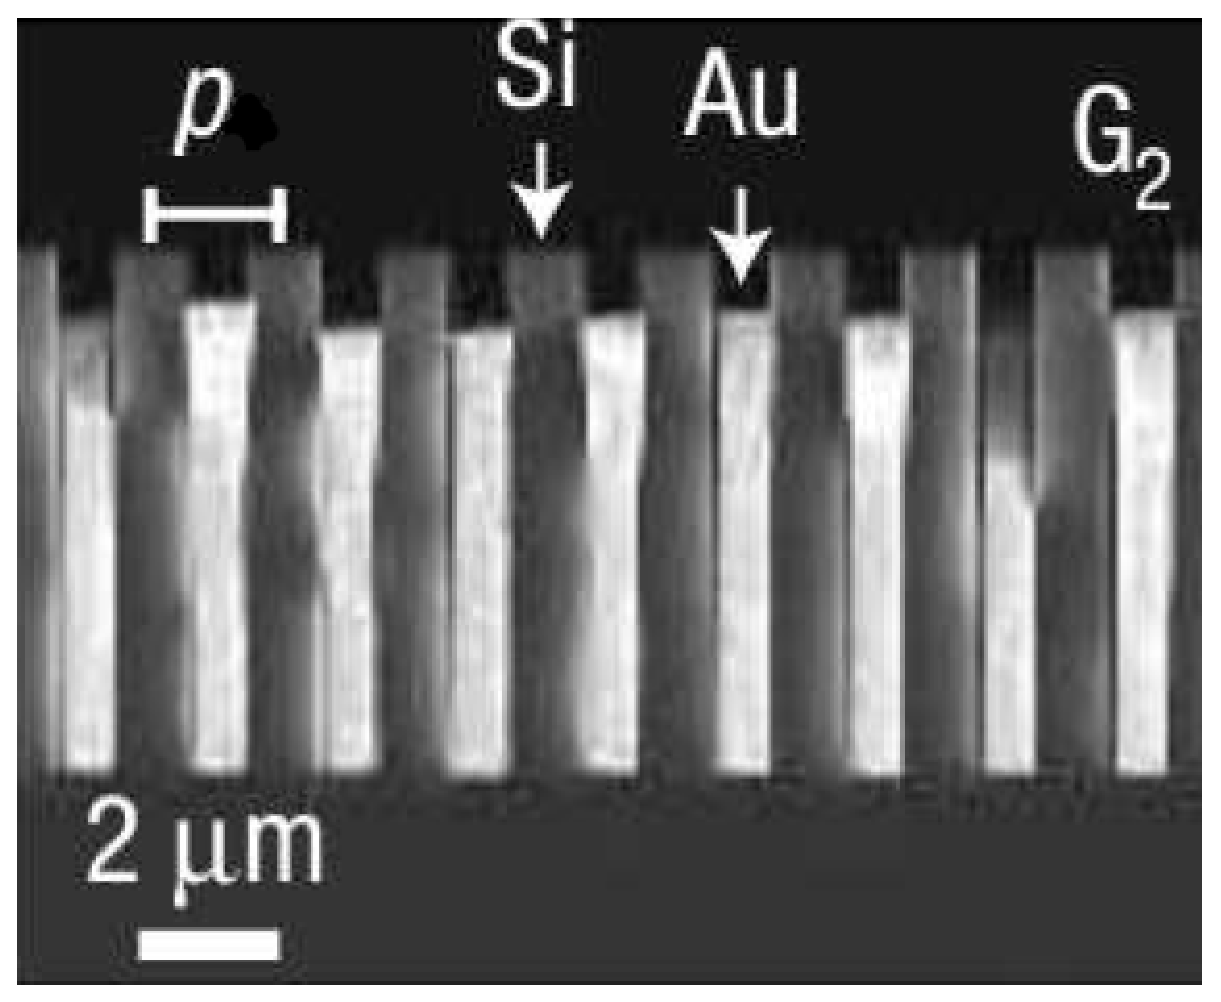
\includegraphics[width=0.45\linewidth]{images/grating.eps}
    \end{figure}
    \begin{itemize}
        \item Optical component with a regular pattern
        \item Used to diffract X-ray beams
    \end{itemize}
\end{frame}


\begin{frame}[c]{Grating Base Interferometer}
    \begin{figure}
        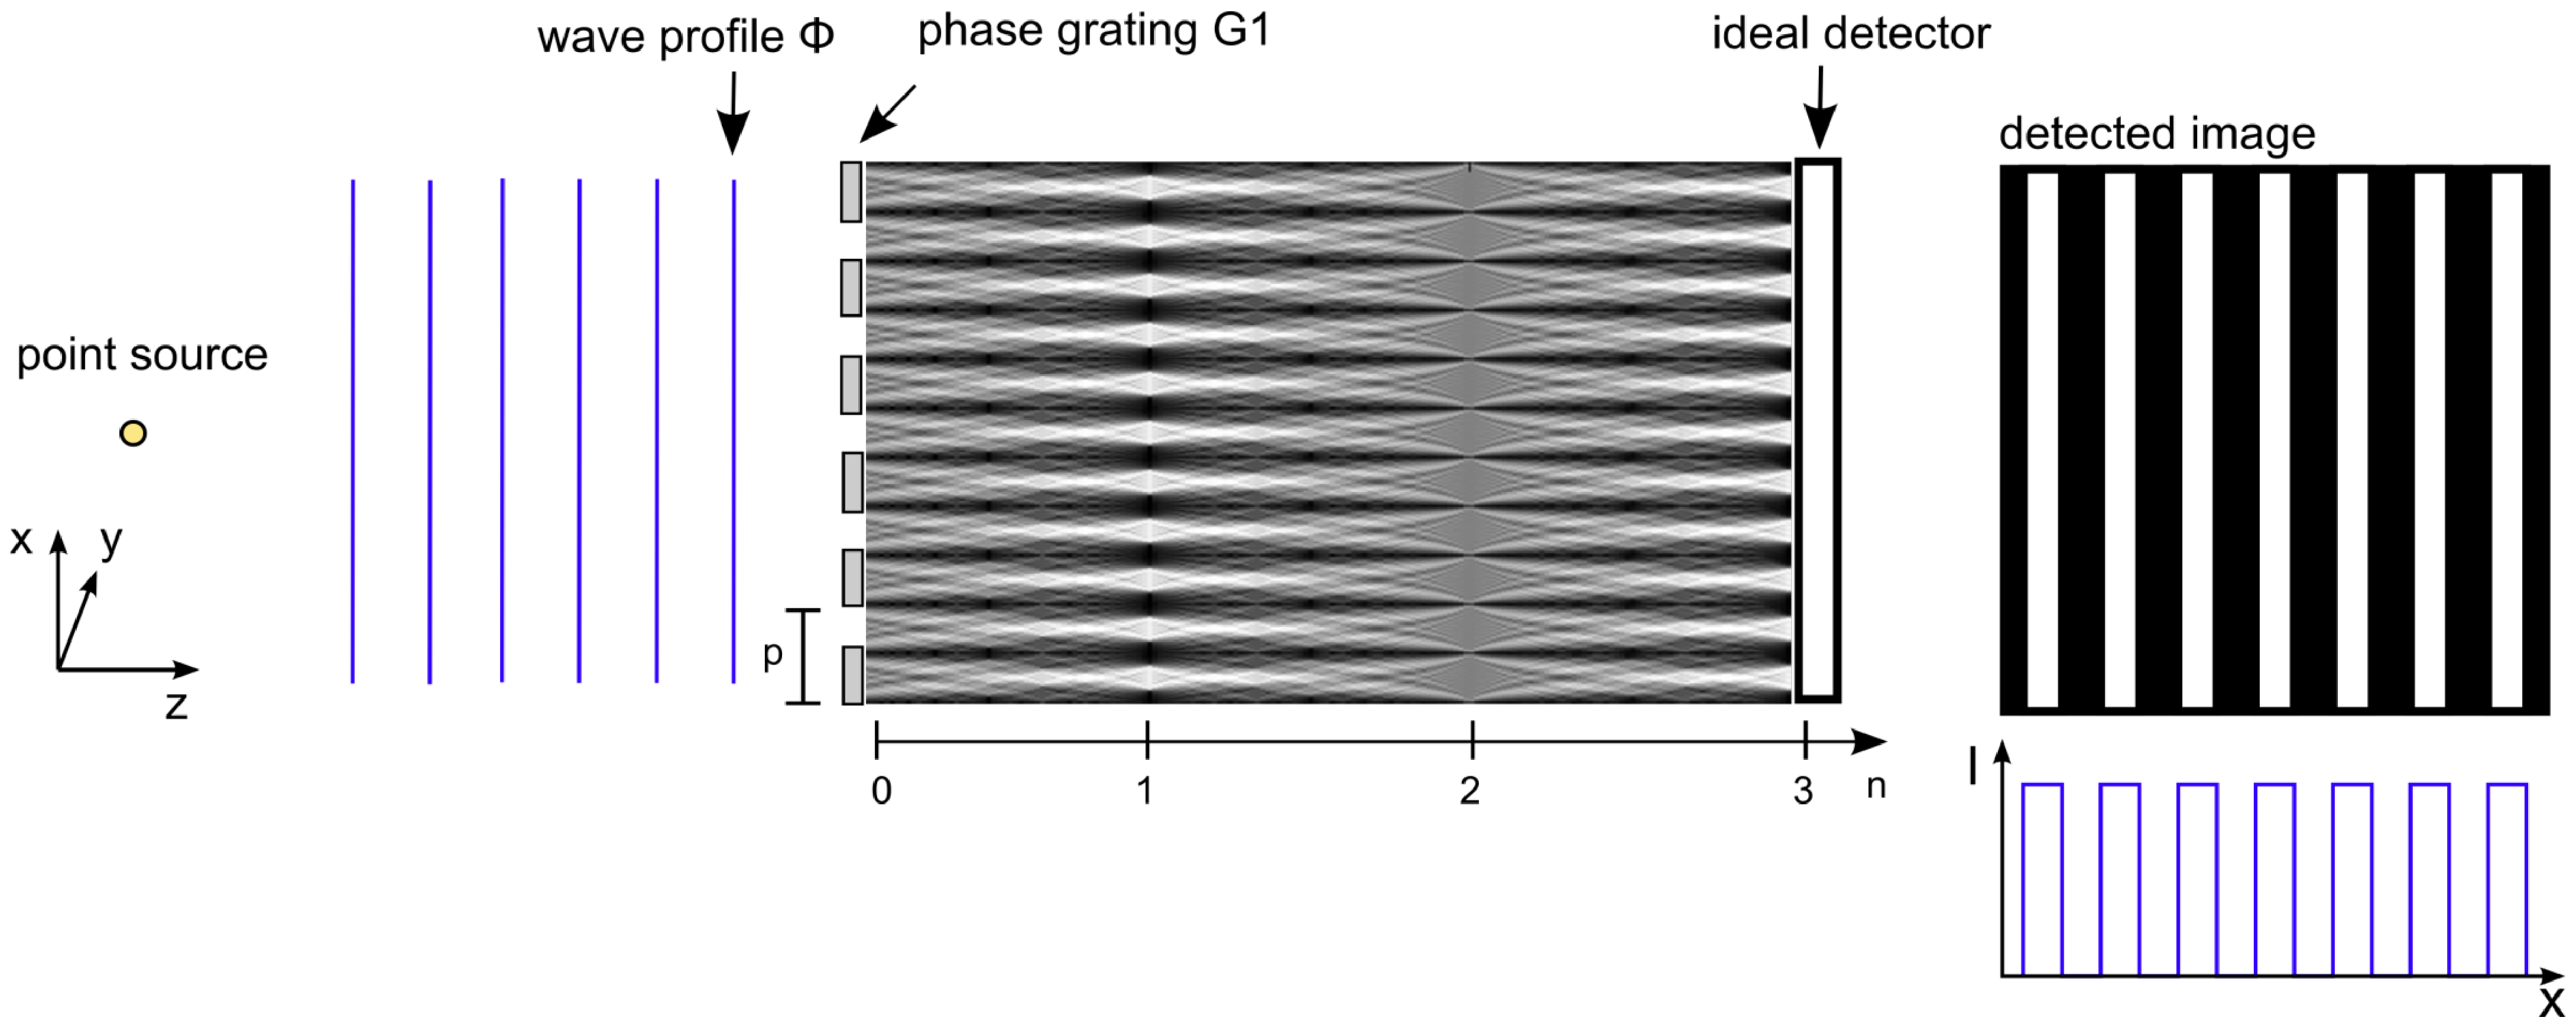
\includegraphics[width=\linewidth]{images/grabase.eps}
    \end{figure}
    \begin{flushright}
        \scriptsize Sources: Wilhelm Haas
    \end{flushright}
\end{frame}


\begin{frame}{Grating Base Interferometer}
    \begin{figure}
        \includegraphics[width=\textwidth]{images/grasebase2.pdf}
    \end{figure}
    \begin{flushright}
        \scriptsize Sources: Wilhelm Haas
    \end{flushright}
\vspace{-1.5cm}
    This pattern is observed for a specific design energy of the interferometer.
\end{frame}

\begin{frame}{Fringe Shifts}
    \begin{figure}
        \includegraphics[width=0.8\linewidth]{images/frigeshift.pdf}
    \end{figure}
    \begin{flushright}
        \scriptsize Sources: Wilhelm Haas
    \end{flushright}
\end{frame}

\begin{frame}[c]{Detector Resolution}
    \begin{figure}
        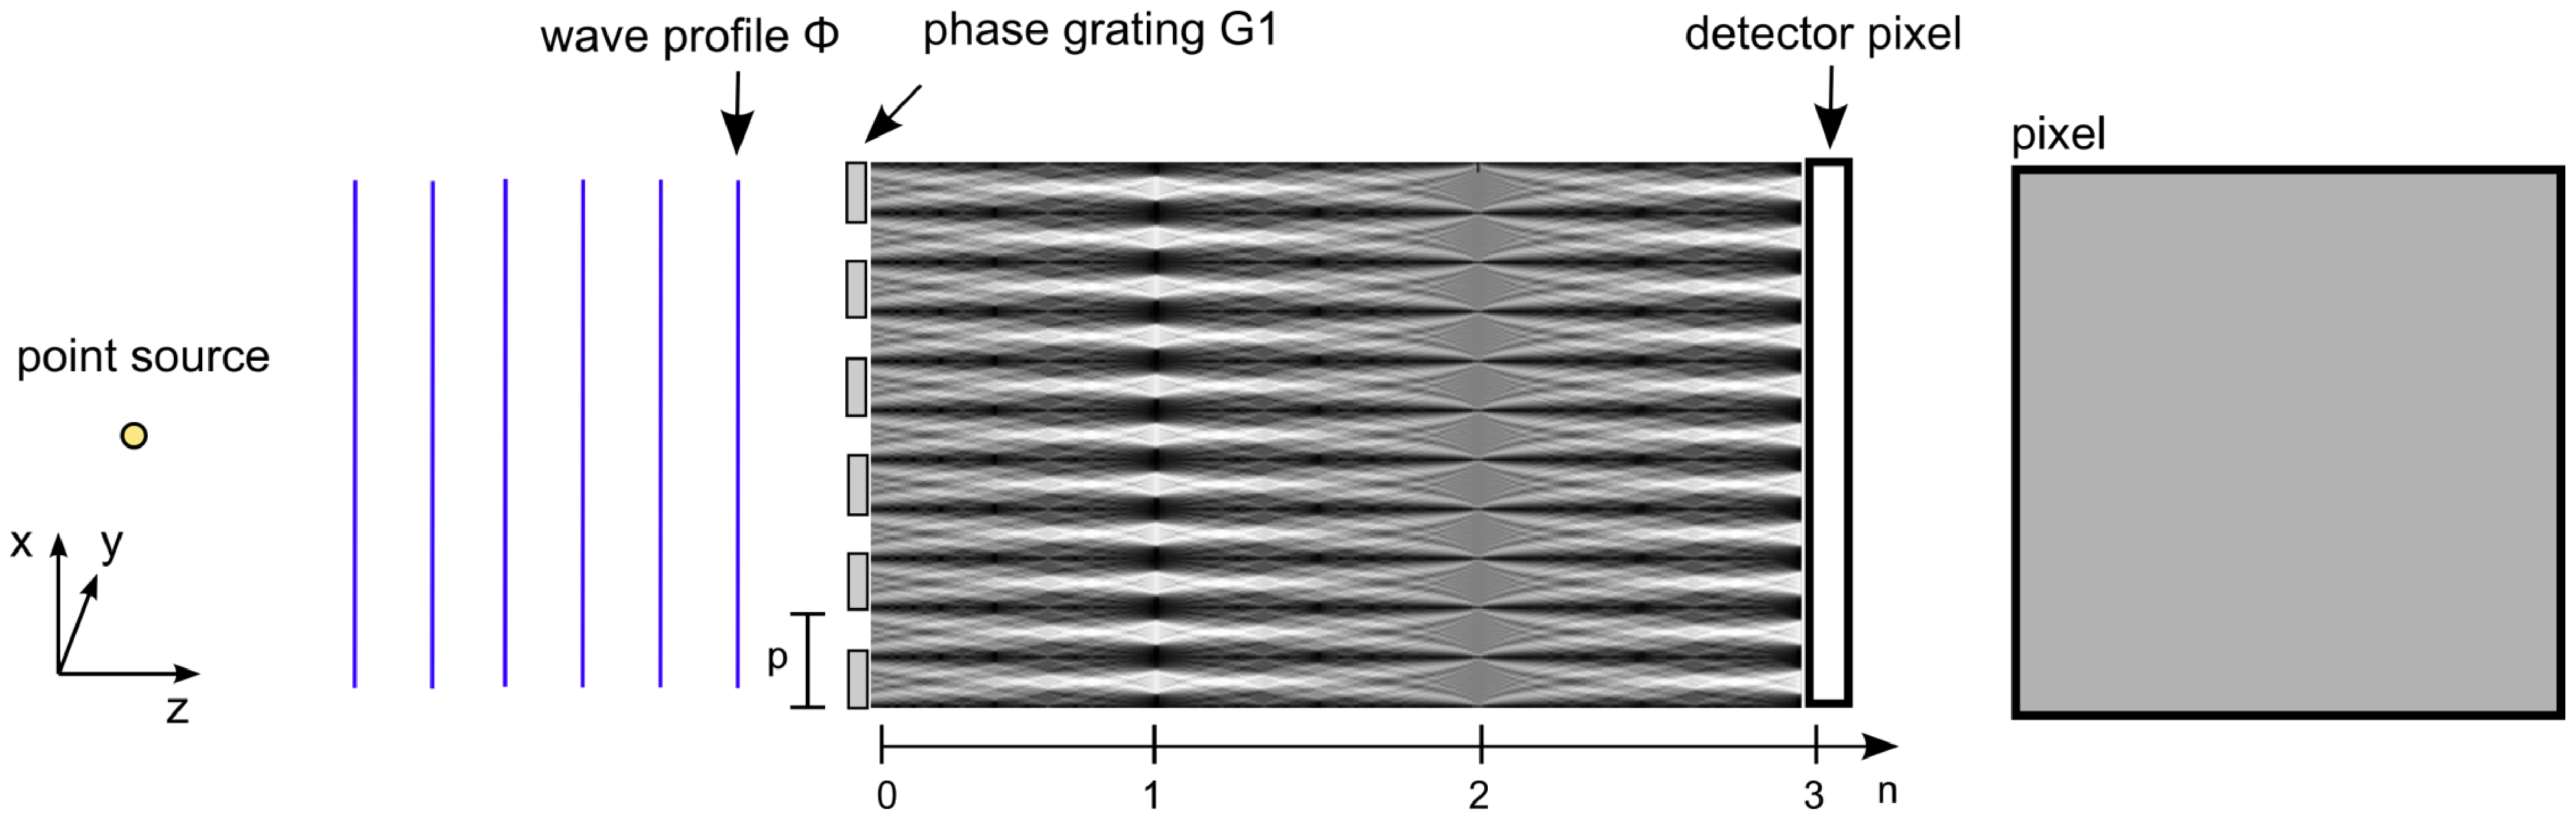
\includegraphics[width=\linewidth]{images/detector.eps}
    \end{figure}
    \begin{flushright}
        \scriptsize Sources: Wilhelm Haas
    \end{flushright}
    Detector pixel presents a single pixel on the detector.
\end{frame}

\begin{frame}[c]{Analyzer Grating G2}
    \bluefat{Problem:}
    \begin{itemize}
        \setlength\itemsep{0.3cm}
        \item Each fringe has a width of few microns\\
              \bluefat{$\Rightarrow$} Detector is not able to resolve each single fringe

    \end{itemize}
    \vspace{0.5cm}

    \bluefat{Solution:}
    \begin{itemize}
        \item Introduction of the \textit{Analyzer Grating G2}
        \item G2 has the same period as the fringes at the design energy
        \item Measured intensities encode different information
              \begin{itemize}
                  \item Absorption
                  \item Phase
                  \item Dark-field
              \end{itemize}
        \item Separation with \textit{phase stepping}
    \end{itemize}
\end{frame}

\begin{frame}{Phase Stepping}
    \vspace{-0.5cm}
    \begin{figure}
        \includegraphics[height=0.92\textheight]{images/phase1.eps}
    \end{figure}
    \begin{flushright}
        \scriptsize Sources: Wilhelm Haas
    \end{flushright}
\end{frame}

\begin{frame}{Phase Stepping}
    \vspace{-0.5cm}
    \begin{figure}
        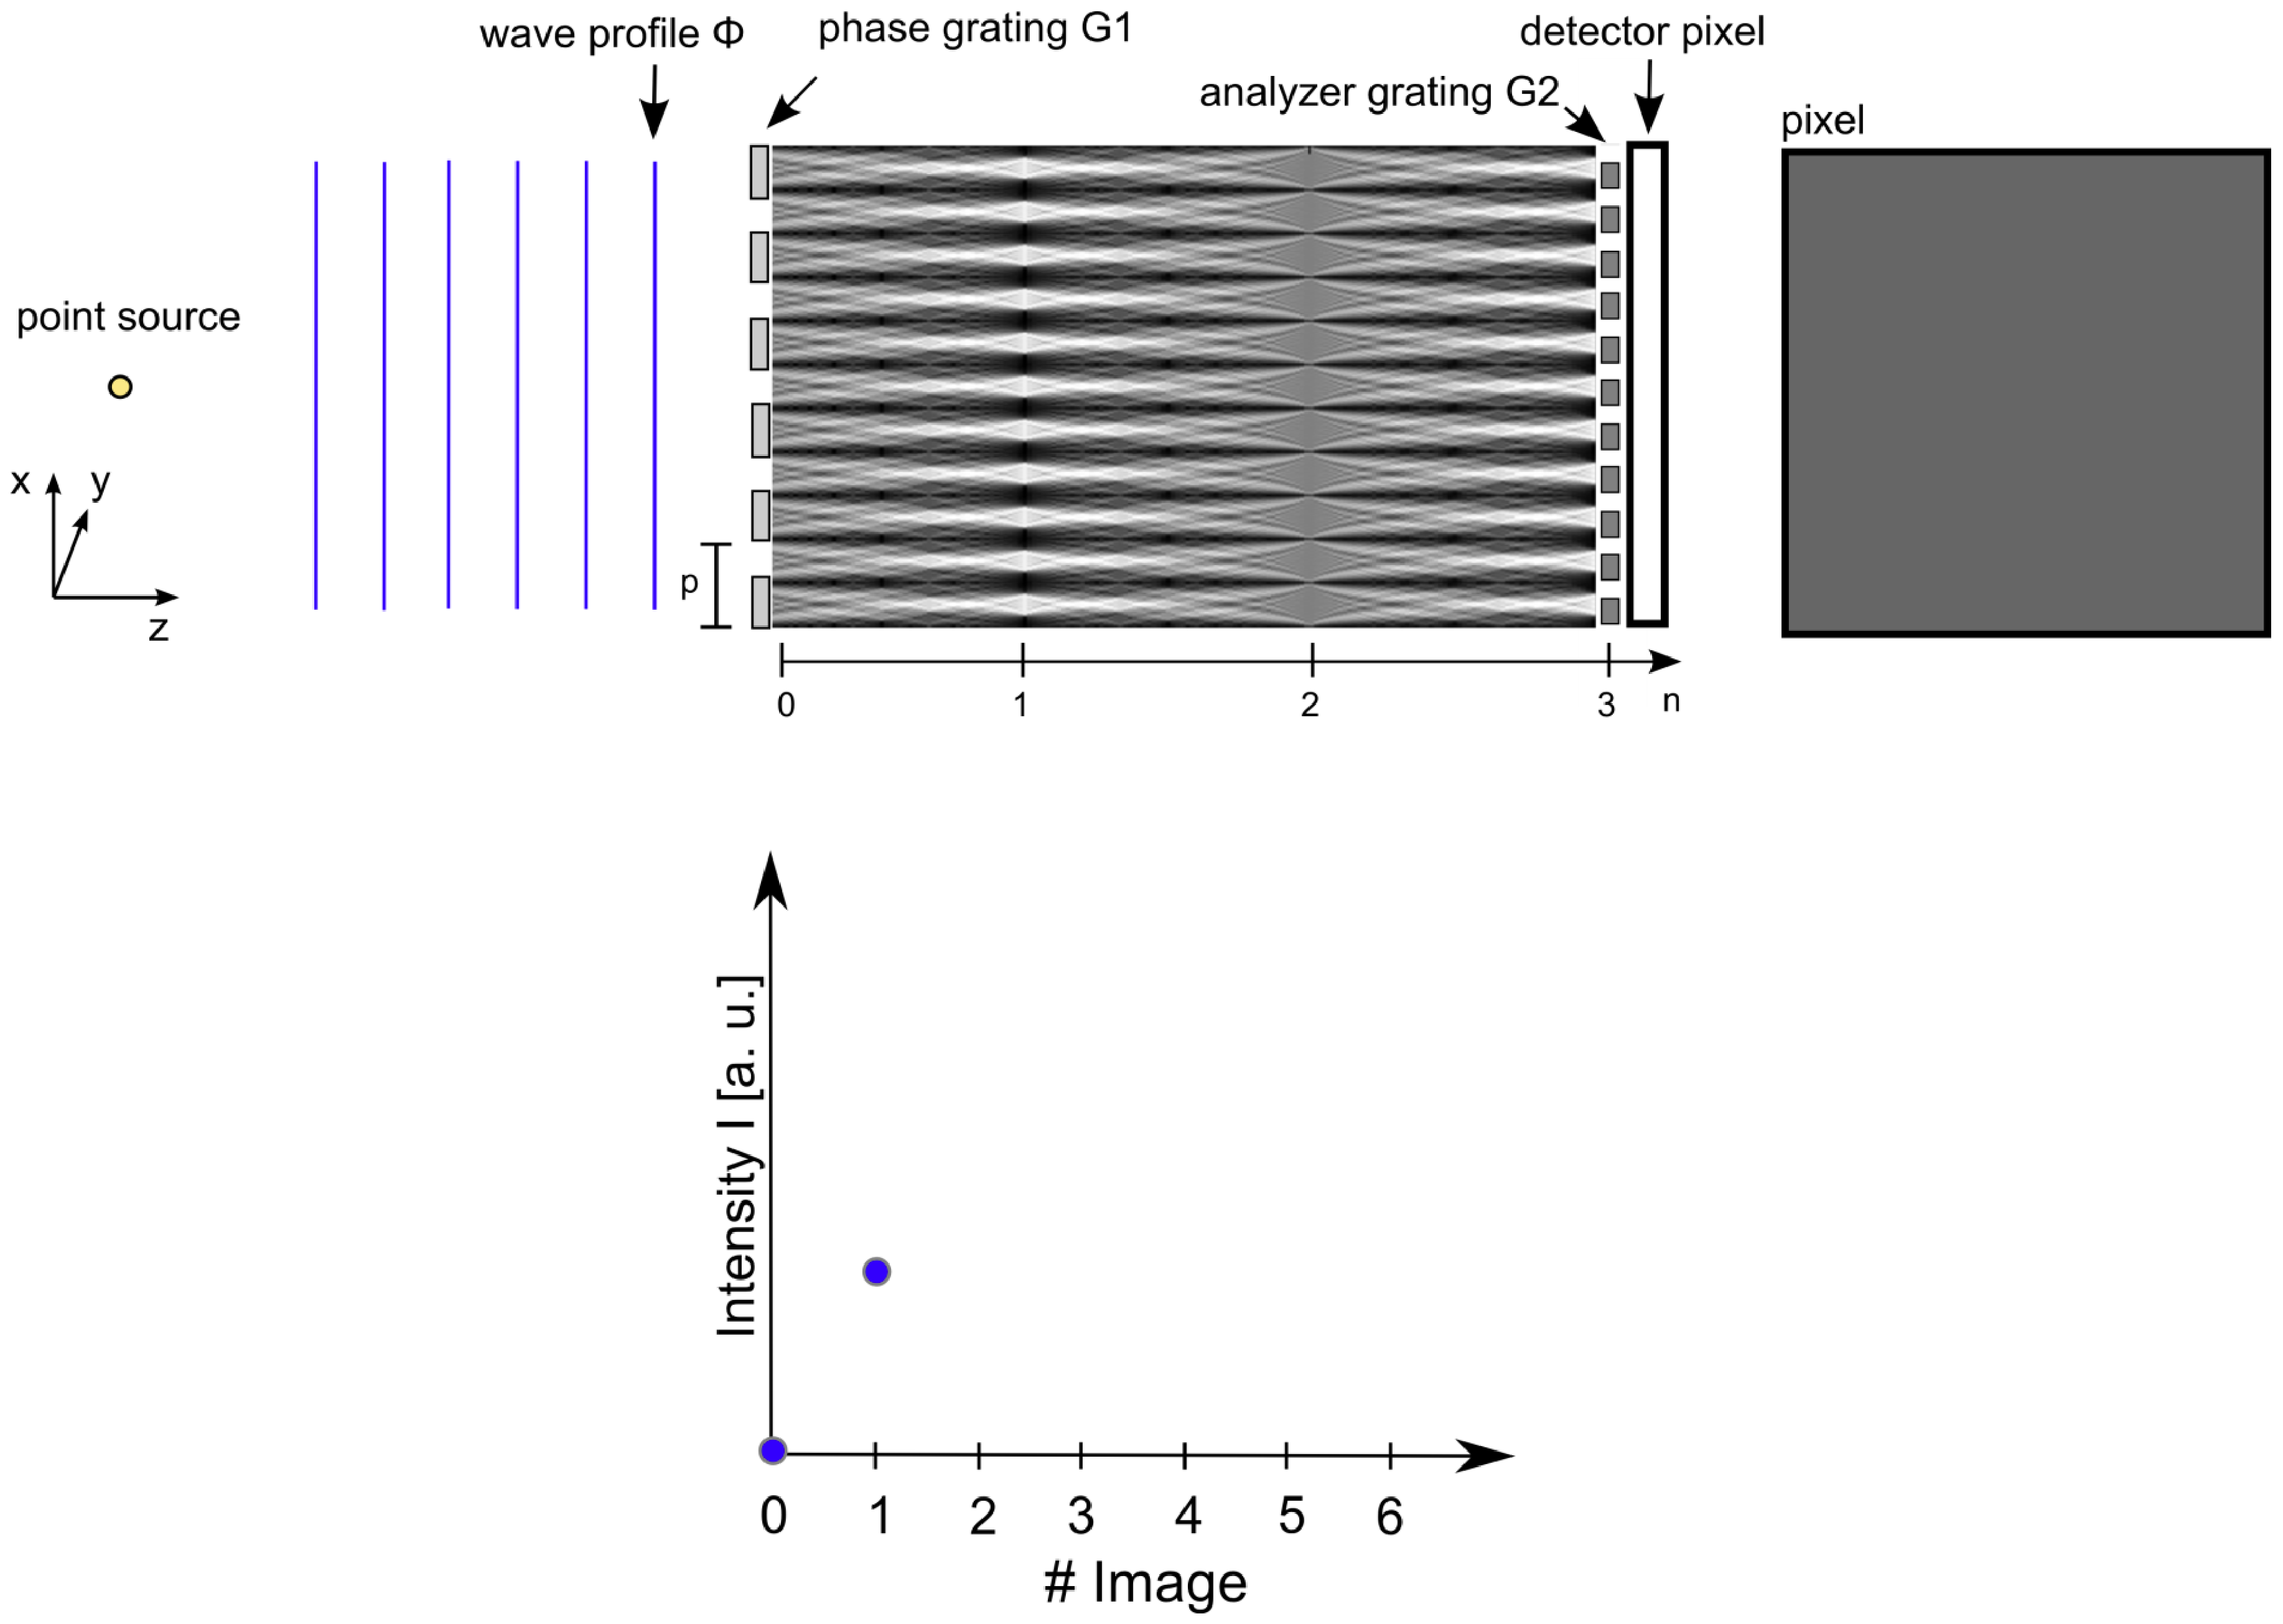
\includegraphics[height=0.92\textheight]{images/phase2.eps}
    \end{figure}
    \begin{flushright}
        \scriptsize Sources: Wilhelm Haas
    \end{flushright}
\end{frame}

\begin{frame}{Phase Stepping}
    \vspace{-0.5cm}
    \begin{figure}
        \includegraphics[height=0.92\textheight]{images/phase3.eps}
    \end{figure}
    \begin{flushright}
        \scriptsize Sources: Wilhelm Haas
    \end{flushright}
\end{frame}

\begin{frame}{Phase Stepping}
    \vspace{-0.5cm}
    \begin{figure}
        \includegraphics[height=0.92\textheight]{images/phase4.eps}
    \end{figure}
    \begin{flushright}
        \scriptsize Sources: Wilhelm Haas
    \end{flushright}
\end{frame}

\begin{frame}{Phase Stepping}
    \vspace{-0.5cm}
    \begin{figure}
        \includegraphics[height=0.92\textheight]{images/phase5.eps}
    \end{figure}
    \begin{flushright}
        \scriptsize Sources: Wilhelm Haas
    \end{flushright}
\end{frame}

\begin{frame}{Phase Stepping}
    \vspace{-0.5cm}
    \begin{figure}
        \includegraphics[height=0.92\textheight]{images/phase6.eps}
    \end{figure}
    \begin{flushright}
        \scriptsize Sources: Wilhelm Haas
    \end{flushright}
\end{frame}

\begin{frame}{Phase Stepping}
    \vspace{-0.5cm}
    \begin{figure}
        \includegraphics[height=0.92\textheight]{images/phase7.eps}
    \end{figure}
    \begin{flushright}
        \scriptsize Sources: Wilhelm Haas
    \end{flushright}
\end{frame}



\begin{frame}{Incoherent polychromatic X-Ray Source}
    \vspace{-0.5cm}
    \begin{figure}
        \includegraphics[width=0.75\linewidth]{images/inco-updated2.eps}
    \end{figure}
    \begin{itemize}
        \item G0 splits the large source in an array of smaller subsources
        \item each sub-source is small enough to create an interference pattern
    \end{itemize}
\end{frame}

\begin{frame}{Formulas}

    \vspace{-0.5cm}
    \begin{minipage}{0.5\textwidth}
        \begin{figure}
            \includegraphics[width=0.9\linewidth]{images/formula.pdf}
        \end{figure}
    \end{minipage}\begin{minipage}{0.5\textwidth}
        \begin{itemize}
            \setlength\itemsep{-0.2cm}
            \item \textbf{\color{faublue}{Differential phase image}}
                  \begin{eqnarray*}
                      \Delta \phi = \phi_{ff} - \phi_o = \dfrac{\lambda d}{p_2} \dfrac{\partial\Phi}{\partial x}
                  \end{eqnarray*}

            \item  \textbf{\color{faublue}{Attenuation}}
                  \begin{eqnarray*}
                      \mu = - \text{ln} \left( \dfrac{\text{mean} ( I_{o}(x_p))}{\text{mean} ( I_{ff}(x_p))} \right)
                  \end{eqnarray*}

            \item \textbf{\color{faublue}{Visibility (contrast), n=\{off, o\}}}
                  \begin{eqnarray*}
                      V_n = \dfrac{\max(I_n(x_p)) - \min(I_n(x_p))}{\max(I_n(x_p)) + \min(I_n(x_p))}
                  \end{eqnarray*}

            \item \textbf{\color{faublue}{Dark-field}}
                  \begin{eqnarray*}
                      D = \dfrac{V_{ff}}{V_{o}}
                  \end{eqnarray*}
        \end{itemize}
    \end{minipage}
\end{frame}


\section{Summary: X-ray Dark-field Imaging}%
\label{sec:further_reading}

\begin{frame}[c]{X-ray Dark-field Imaging}
    \begin{itemize}
        \large
        \setlength\itemsep{0.3cm}
        \item<1-> Caused by ultra-small angle scattering
        \item<2-> Allows reconstruction of structures at length scales below
              the resolution of conventional X-ray imaging systems.
        \item<3-> Yields the possibility of reconstructing the orientation of fibrous structures
        \item<4-> May become medically useful, i.e. diagnosis of osteoporosis

    \end{itemize}
\end{frame}

\section{Examples}%
\label{sec:examples}

\begin{frame}[c]{Examples -- Frozen mouse}
    \begin{center}
        \begin{tabular}{ll}
            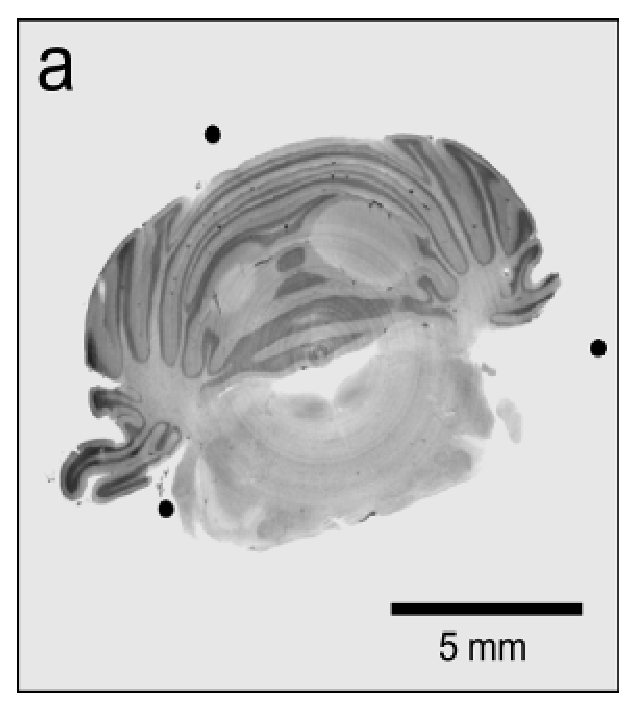
\includegraphics[width=0.3\linewidth]{images/brainrat1.eps} & 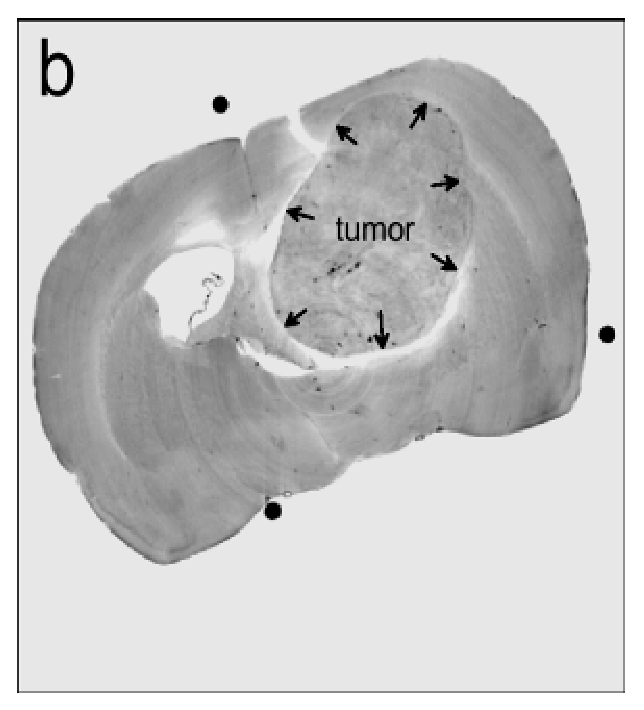
\includegraphics[width=0.3\linewidth]{images/brainrat2.eps}
        \end{tabular}
    \end{center}

    \begin{center}
        \begin{flushright}
            \scriptsize Sources: Frank Pfeiffer TU M\"uchen
        \end{flushright}
    \end{center}
\end{frame}

\begin{frame}[c]{Examples -- Gummi Bears}
    \begin{center}
        \centering{}
        \includegraphics[width=\textwidth]{images/gummi.png}
    \end{center}

    \begin{center}
        \begin{flushright}
            \scriptsize Courtesy of ECAP Erlangen~\cite{bopp18}
        \end{flushright}
    \end{center}
\end{frame}

\begin{frame}{Examples -- Dark-field: Chicken Wing}
    \begin{center}
        \begin{tabular}{ll}
            absorption:                                             & dark-field:                                             \\
            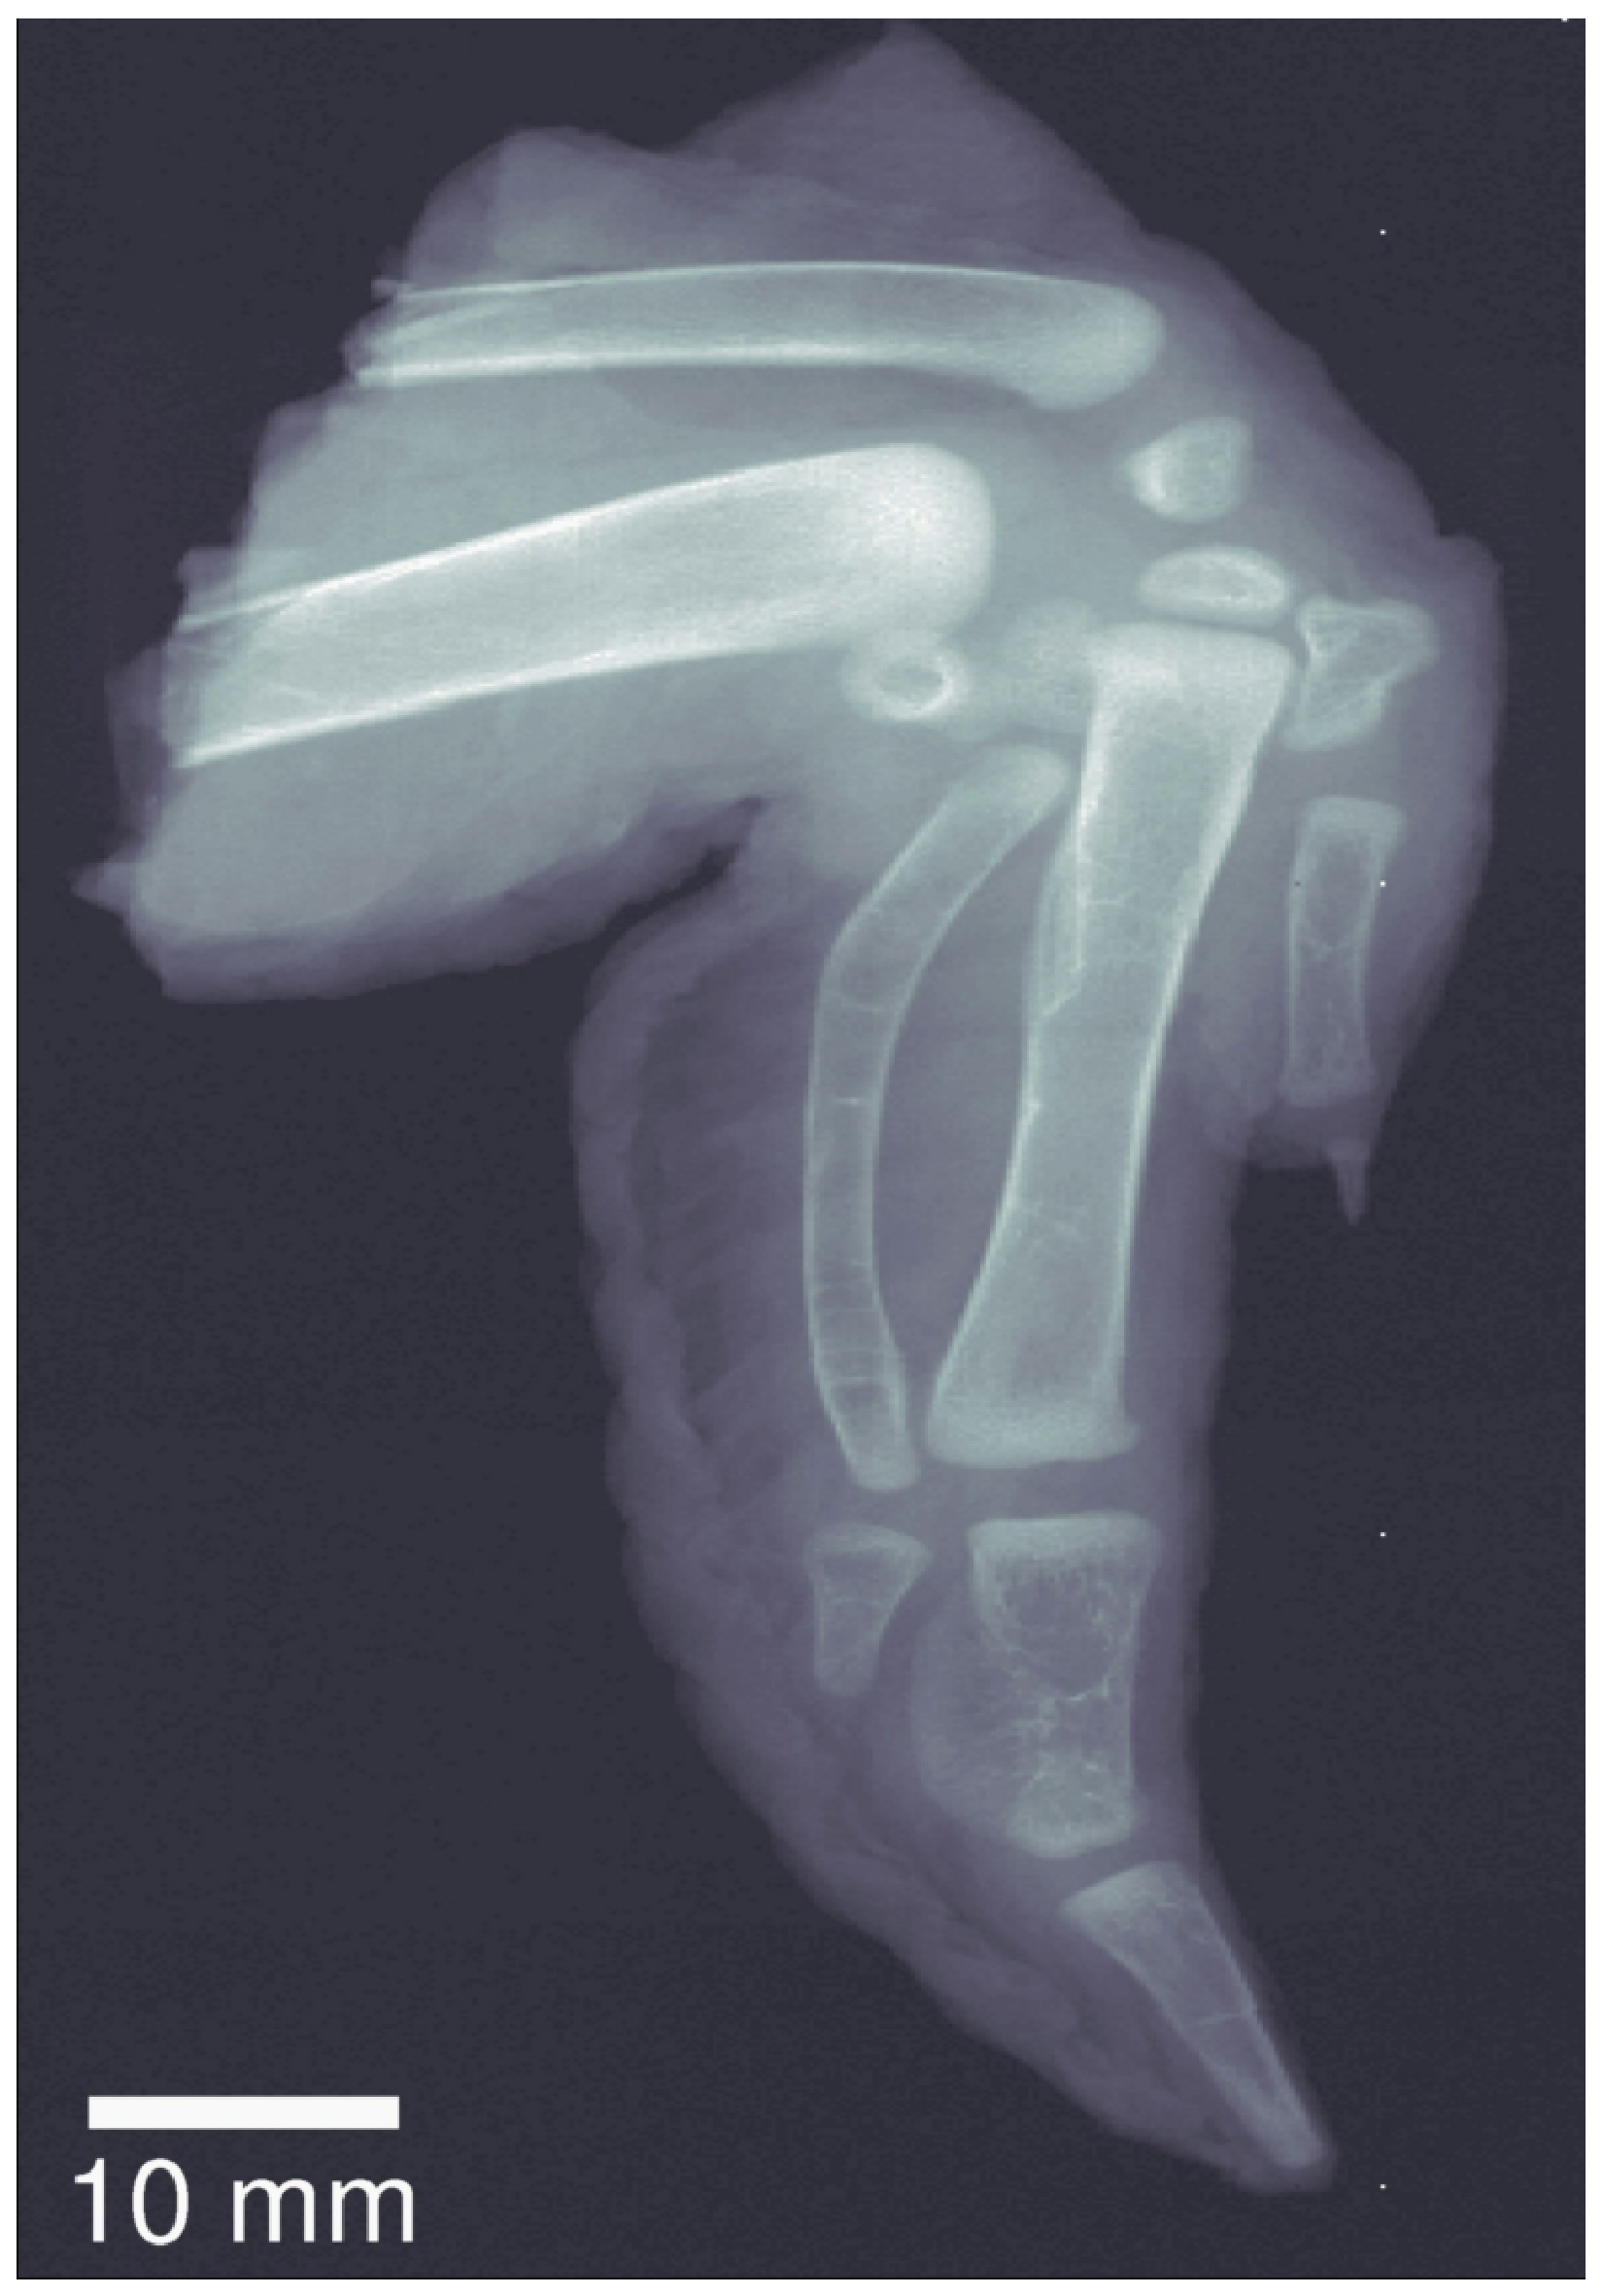
\includegraphics[width=0.25\linewidth]{images/wing1.eps} & 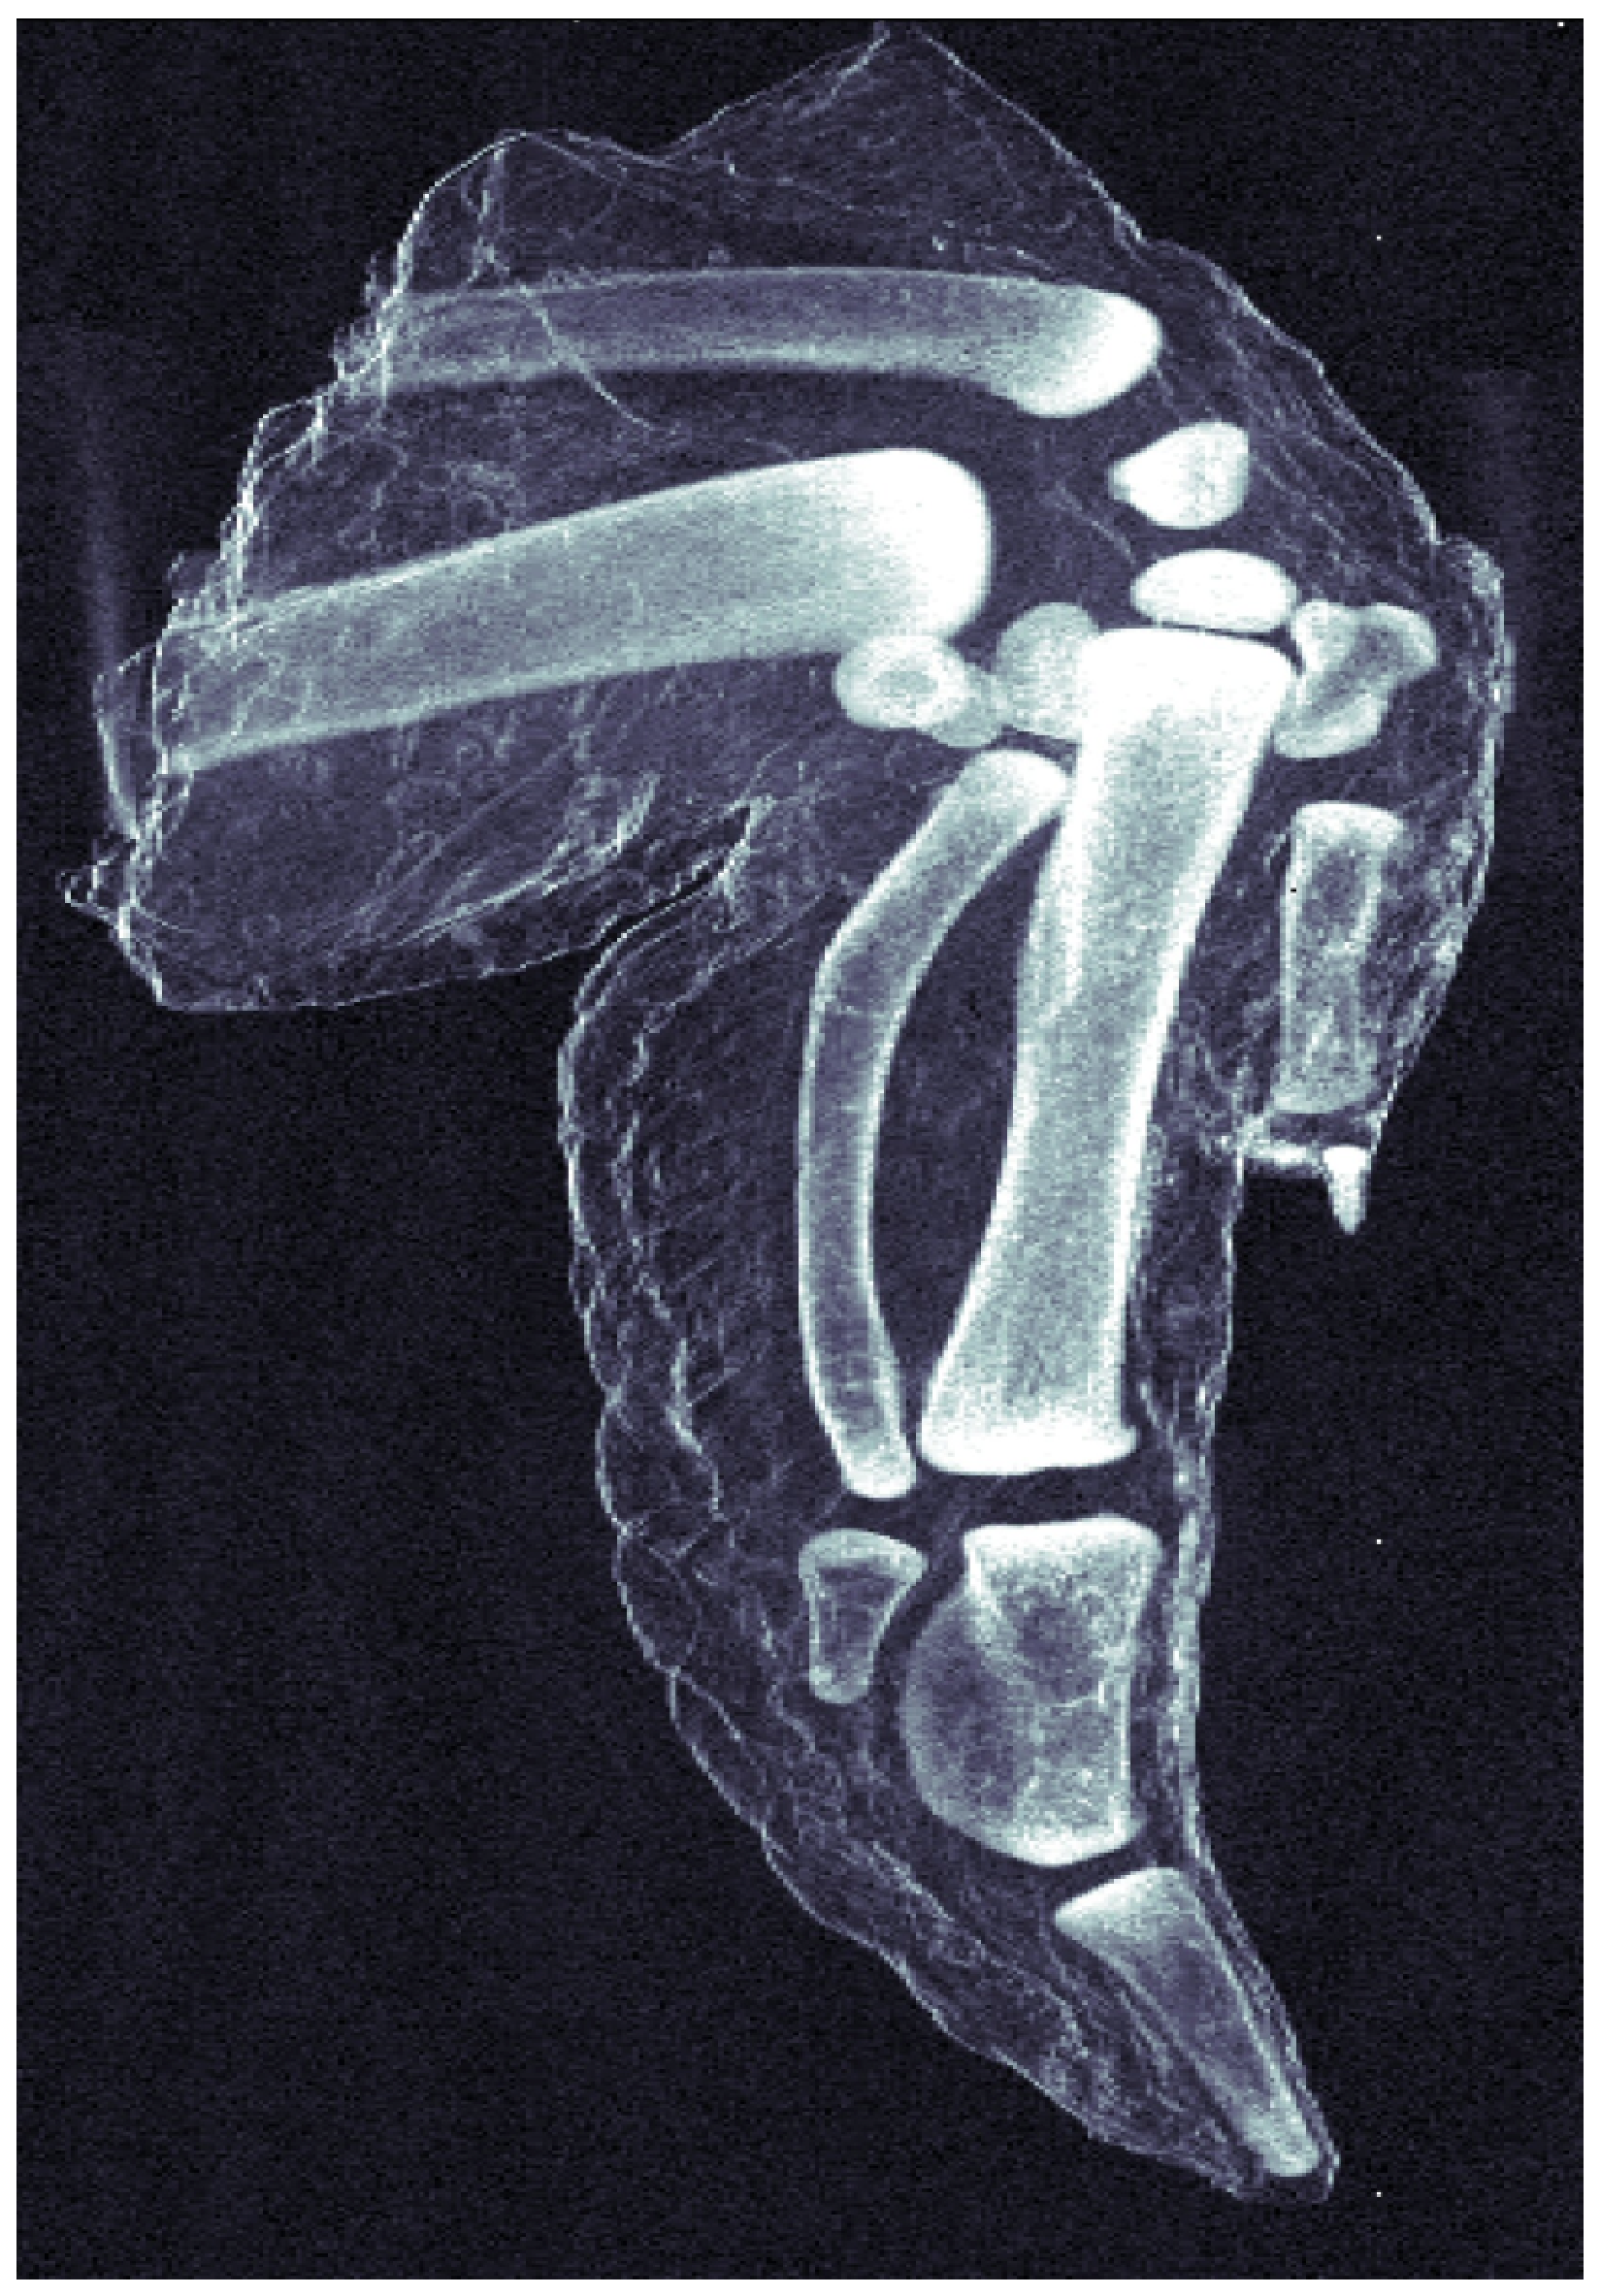
\includegraphics[width=0.25\linewidth]{images/wing2.eps}
        \end{tabular}
    \end{center}
    \begin{center}
        \begin{flushright}
            \scriptsize Sources: Frank Pfeiffer TU München
        \end{flushright}
    \end{center}
\end{frame}
\begin{frame}{Examples -- Dark-field Reconstruction: CFRC sample}
    \begin{center}
        \begin{tabular}{ll}
            Dark-field reconstruction                              & Visualization of CFRC sample:                                          \\
            \includegraphics[height=0.75\textheight]{images/CFRC.pdf} & \includegraphics[height=0.75\textheight]{images/microstructures_cfrc.pdf}
        \end{tabular}
    \end{center}
\end{frame}

\begin{frame}{Examples -- Dark-field Reconstruction: Wooden block}
    \begin{figure}
        \centering
        \includegraphics[width=0.6\linewidth]{images/Wooden.pdf}
        \caption[Visualization of micro-structures of the wooden sample.]{Visualization of micro-structures of representative layer of the wooden sample. \label{images:Wooden3D}}
    \end{figure}
\end{frame}

\begin{frame}{Examples -- Experimental Setup in ECAP}
    \begin{center}
        \begin{tabular}{l}
            Experimental Setup in ECAP \\
            \includegraphics[width=0.5\linewidth]{images/setup.pdf}
        \end{tabular}
    \end{center}
    \begin{flushright}
        \scriptsize Sources: Erlangen Centre for Astroparticle Physics (ECAP), Erlangen, Germany
    \end{flushright}
\end{frame}

\section{Further Questions?}

\begin{frame}[t]{Further Readings}
    \begin{itemize}
        \item \fullcite{bopp18}
    \end{itemize}

\end{frame}

\end{document}
